% Basic document class
\documentclass[landscape, twocolumn, 12pt]{article}

% General public packages loaded here:
\usepackage{amsmath}
\usepackage{amssymb}
\usepackage{graphicx}
\usepackage{caption}
\usepackage{float}
\usepackage{pdfpages}
\usepackage{gensymb}
\usepackage{tikz}
\usepackage{forest}
\usetikzlibrary{decorations.pathmorphing}
\usetikzlibrary{decorations.markings}
\usetikzlibrary{backgrounds}

% To-do list
\usepackage{enumitem,amssymb}
\newlist{todolist}{itemize}{2}
\setlist[todolist]{label=$\square$}

 
\setcounter{tocdepth}{2}
%\usetikzlibrary{math}

\usepackage[toc,page]{appendix}

% Custom .sty files loaded here:
\usepackage{../TitlePage}
\usepackage{../mathshortcuts}
\usepackage{../stanli}

% Add item to glossary
% Check mathshortcuts.sty for documentation
% Uncomment following example line to add more items
%\glo{Mu}{M_{u}}{Factored ultimate moment in the beam}

% Title Page commands
% Check TitlePage.sty for documentation

% Fill out the following information
% This is used by TitlePage.sty
\title{Contributing to gitMechanics}
\subtitle{Basics of \LaTeX{}, git, and How You Can Help}
\coursenum{GIT101}
\coursetitle{INTRODUCTION TO GIT}
\university{Arizona State University}

% Path to title page figure.
% If note specified the default image will be used.
\titleimage{../assets/images/gitMechanics}
\author{Brian Chevalier}
\date{\today}

%-------------------------------------------
\begin{document}

% Leave this alone. 
% It will make the title page
\maketitle

% I'm not content with the name abstract
% but whatever...
\renewcommand{\abstractname}{Welcome to the gitMechanics Team!}

\begin{abstract}
This document is a beginners introduction to the information needed to contribute to gitMechanics. We will cover the basics of git, \LaTeX{}, and we'll end on the steps you need to take to make a contribution.

All suggestions, corrections, or new material is very welcome, no matter how small. The \textit{beauty} of open-source is that all contributions make a permanent difference. If you have no experience with any of these things don't be intimidated! Feel free to reach out for any clarification or help you need. I'm so happy you've even considered helping.
\end{abstract}

% Add additional sections here
\section{Introduction to git}

Git is an open-source, distributed \textit{version control system} originally built by Linus Torvalds for managing contributions to Linux. Git is now one of the world's most used version control systems (all of Windows is now managed with git), one of the primary places git repositories are stored is on github.com (which is where this document lives). At it's core all git does is keep track of changes in files, but particularly plain text files. Plain text files can have many file extensions such as txt, md, tex, etc. We'll talk about these more later.

Git can be used through two primary ways: via a graphical user interface (GUI) or through the command line. Git is available on all platforms (even iOS, Android, and chromeOS. On iOS I highly recommend Working Copy). Before we talk about actually using git we'll look at some basic terminology.


\subsection{Vernacular}

There are a few concepts that you'll want to understand in general before getting started with the particulars of using git. Some of these words can be very confusing for beginners so we're going to lay out some words that you'll want to be familiar with.

\begin{description}
	\item[Repository] Also called a ``repo''. This is a directory that stores your source files. There is a special folder called ``.git'' which contains the metadata about the repo. Folders that start with a dot will be hidden in most files systems.
	\item[Clone] When you see a project on github you can clone that project. This is a full copy of a repository. Every repo is a clone which is why git is a distributed version control system.
	\item[Fork] A fork is a copy of a repo that is associated with your github account. This gives you a repo that you can edit and push changes to. Typically you will \textit{fork} someone's repo on github.com, then \textit{clone} that repo to your local machine. In effect, all repos are clones and forks because it is a distributed network.
	\item[Commit] After you make changes to a repo you'll want to commit those changes. This is essentially like a bookmark in your repo that holds the state of your repo. Every commit must be made with a message (make sure it's useful!) and optional additional comments.
	\item[Stage] Before you actually make a commit you will will have to ``stage'' or decide which files will be included with the commit. If you're using a GUI git tool this may just be a step while making a commit. On the command line you have to stage the files you are going to commit (this is done with git add filename or git add -a for all files in the repo to be added) and then commit them.
	\item[Fetch] When you're working with a repo you typically have a version of that repo on a server that you want to route your changes through. If someone else has made changes to that repo or you made changes on another device you have to fetch changes, then merge them into your repo and push those changes back to the server.
	\item[Push] You push changes to a server. You can push multiple commits at a time, so you don't have to push every time you make a commit or change a file.
	\item[Pull] A pull is a combination of fetch and merge. You'll typically want to avoid pulling changes into your repo because you want to manually fetch and then merge in changes.
	\item[Pull Request] This is a request made by someone to suggest changes to a repo that they do not have write access to. This is very common for open source projects so changes to the canonical source code is vetted by project maintainers.
	\item[Branch] A repo starts with one branch called the master. You can create as many branches as you want. For instance, you may want to make a new branch that includes 
	\item[Merge Conflict] This is the error that occurs when two that git attempts to combine have different text on the same line number that it cannot reconcile. This requires manual fixing but does not often happen.
	\item[Diff] A diff is to show the differences between two or more files. Depending on your knowledge, a GUI is likely better for seeing diffs since it will be easier to understand.
	\item[Checkout] The power of git is that you can checkout previous commits of a repo. As long as all the files in your repo are already committed, you can checkout another branch or another commit. This eliminates the fear of making destructive changes. As long as you commit changes regularly and make descriptive commit messages you will always be able to return to a known change.
	\item[Cherrypick] Sometimes when you're working with multiple branches you'll want to choose a commit from one branch and apply it onto another. This is what a cherrypick does. You will not likely need to do this.
	%\item[Rebase]
\end{description}

\subsection{Git on the Command Line}

If you choose to use a command line tool for git it is very important you understand what these words mean as many of them are the names of commands you'll want to use when managing your repo. The most common are clone, add, commit, fetch and push. The typical steps you make when working on a repo is: clone someone else's repo. Make changes. Fetch changes from the server to see if any changes have been made there and merge in the changes. Add your files to a commit, then make the commit. Finally, you can push your files to the server. This can be accomplished by the following commands:

\begin{lstlisting}[language=bash]
	git clone [URL]
	git fetch
	git merge
	git add --all
	git commit -m "commit message"
	git push
\end{lstlisting}

Note that you'll want to replace [URL] with the URL of the repo that you are cloning. You will enter each line for each part of the process.

Here is a great video on YouTube with an in depth example on using git from the command line. Even if you don't use the command line it is great for understanding how git works.
\begin{center}
	\url{https://youtu.be/0fKg7e37bQE}
\end{center}

\subsection{GUI git Clients}
Many text editors include git integration out of the box including MATLAB and VSCode. 

Github provides a GUI client for users on macOS and Windows:
\begin{center}
\url{https://desktop.github.com}
\end{center}

and provides full guides on using their application:
\begin{center}
	\url{https://help.github.com/desktop/guides/}
\end{center}


\subsection{Making a Pull Request}

Now we will take a look at making a \textit{pull request}. A pull request is your method of suggesting changes to someone's work. Typically, big open-source projects are not just a Wikipedia-style free-for-all. Only project maintainers have \textit{write access} to the canonical version of Python, for instance. However, community members \textit{are} able to fork a copy of the repository to their own github. This allows write access to your own version of the repo. After you make changes to your code, you can then make a pull request on the original repo. This ensures that the code can be vetted by automated testing (i.e. continuous integration), and further tested by humans.

The following video shows how to fork a public repo, make changes to that repo where you have write access, then suggest changes via a pull request to a project.

\begin{center}
	\url{https://youtu.be/YTbRzhQju4c}
\end{center}
\section{Introduciton to \LaTeX{}}
\LaTeX{} (pronounced lay-teck) is a free, open-source high-quality document preparation system (this document is written and compiled with \LaTeX{}!). \TeX{} was written and designed by Donald Knuth in 1978. \LaTeX{} builds on top of the work of Knuth providing more functionality through a more advanced set of macros.

\subsection{Vernacular}

\begin{description}
	\item[Macro] A macro is a \LaTeX{} command that can take input and does something with it. You can define any number of custom macros (also called commands) that can speed up your document preparation and make your style more consistent.
	\item[Package] A package is a set of predefined \LaTeX{} macros packaged up for your use. Users can create their own packages. gitMechanics relies on a few custom packages.
	\item[Document class] There are many document classes that you can use, and you can even define your own classes. Classes include: article, standalone, beamer (slide presentation format), report, book, etc. Each class provides a set of commands to typeset your work.
	\item[Environments] Text in an environment is processed in a particular way by the compiler. Inside an environment particular types of commands are available for use. The entire body of the document is wrapped in the document environment. There are also list environments, math environments, floating environments, and of course you can define custom environments.
\end{description}

\subsection{Getting \LaTeX{} on Your Machine}
Your first step is to install a distribution of \LaTeX{}. This will be different depending on your platform, however it is available on all platforms (you can use the Linux distribution on ChromeOS. On iOS you can get a dedicated app, I reccomend TeX Writer). The following URL includes links on where to install the different distributions.

\begin{center}
	\url{https://www.latex-project.org/get/}
\end{center}

Most also come with a GUI editor and built in methods for compiling your documents so you don't have to touch the command line. Each editor will be slightly different so you'll have to spend a while getting to know your editor. Note that you can also opt to use your own text editor and compile from the command line using pdflatex. Regardless, make sure your text editor has good code completion support for \LaTeX{} otherwise it will make learning commands a nightmare.


\subsection{Compiling Your First Document}

The most basic document needs two things. First you have to define your ``document class''. As discussed before, there are many classes. Document classes can also take optional inputs in square brackets before the actual document class. This document is an article class document and the options are landscape, twocolumn, and 12pt. The options must be separated by commas. The example code below typsets a blank document. Note that the article declaration is on the second line, which is completely valid, but is also done to fit within the column margins. Also note that your document will be within the document environment, and that the \% sign indicates a comment.

\begin{center}
\begin{latexcode}
\documentclass[landscape, twocolumn, 12pt]
{article}

\begin{document}
% Your document goes here
\end{document}
\end{latexcode}
\end{center}

\subsection{Document Structure}



\subsection{Loading Packages}
Standard \LaTeX{} is good, however, you will likely need to load additional packages to extend the language. You can import a package like the following:

\begin{center}
\begin{latexcode}
\usepackage{amsmath}
\end{latexcode}
\end{center}
You will want to typically use the AMSMath package since it adds many commonly used math symbols. You can find full documentation on the package at:

\begin{center}
	\url{https://www.ctan.org/pkg/amsmath}
\end{center}

The Comprehensive \TeX{} Archive Network (CTAN) has many packages and documentation for packages that are typically already included with your \LaTeX{} distribution. Most packages have the full documentation in PDF format available on CTAN.


\subsection{Equations in \LaTeX{}}
If there's one thing \LaTeX{} is known for it's typesetting math and equations. We're going to get into that now. For math to be added to your document you have to be in some sort of math mode. This means you could be in a math environment or have your math inline with delimiters. 

Math environments include: align, equation, or a few more. Equations in this environment will automatically be centered and numbered. You can suppress numbering of these environments by adding ``*'' after the environment name. The following equation is typeset using the equation environment:

\begin{equation}
	\int_{0}^{L} f(x) dx
\end{equation}

\begin{center}
\begin{latexcode}
\begin{equation}
\int_{0}^{L} f(x) dx
\end{equation}
\end{latexcode}
\end{center}

Note that the braces around the limits of integration are not strictly needed for single character limits, however it is best practice to keep them in braces to avoid confusion and be consistent for more complicated equations.

The next important math environment is the align environment. The align environment allows typesetting multiple consecutive equations aligned. The following is an example of that:

\begin{align}
y &= mx + b\\ 
  &= \frac{\Delta y}{\Delta x}x + b
\end{align}

The syntax looks like:

\begin{center}
\begin{latexcode}
\begin{align}
y &= mx + b\\ 
  &= \frac{\Delta y}{\Delta x}x + b
\end{align}
\end{latexcode}
\end{center}

Things to note: the equations are aligned based on the location of the ``\&'' and new lines are entered with ``\textbackslash''. Greek letters and other commands also require a space after the command name otherwise it will throw an error.

\subsubsection{Lableing and Referencing}

Hyperlinking

\subsubsection{Greek Letters}
Most Greek letters can be included in math mode typically by typing ``\textbackslash'' followed by the name of the letter such as typesetting the letter beta: $\beta$. The following PDF lists many Greek letters and math mode symbols.

\begin{center}
	\url{https://wch.github.io/latexsheet/latexsheet.pdf}
\end{center}



\subsubsection{Operators}
















\section{Drawing in \LaTeX{}}

\LaTeX{} produces truly stunning PDF output, but as the great philosopher, Beyonc\'e once said, ``Pretty Hurts''.

\paragraph{GUI Options}
There are some options to avoid manually marking up drawings. One method is to simply produce figures and drawings in another application, and export as a PDF, or if you like the pixelated compression artifacts, JPEG. You can then save the file in the Figures subdirectory of your project and include something like the following:

\begin{center}
\begin{latexcode}
\begin{figure}[H]
\centerline{
\includegraphics[width=\columnwidth]
{Figures/FIGNAME}}
\caption{CAPTION}
\label{fig:LABEL}
\end{figure}
\end{latexcode}
\end{center}

You can also use a GUI editor that will output to markup formats and include those directly into your source code. You can export to TikZ format which we will discuss in the next section. A great option for this is GeoGebra:

\begin{center}
	\url{https://www.geogebra.org}
\end{center}

\subsection{TikZ}
While including external images works, it can get out of control pretty quickly if you have many figures. It also eliminates the possibility of using a set of macros to keep drawings consistent throughout many documents. Using generated TikZ still runs into this problem. Therefore, the only good option is to learn TikZ markup. For gitMechanics, I have already begun building a library of macros that will hopefully make the processs more straight-forward and consistent between documents.

The following site has many example TikZ examples:

\begin{center}
\url{http://www.texample.net/tikz/examples/}
\end{center}



\subsubsection{TikZ Math}
The TikZ Math library is a great way to use math to better geometrically describe your diagrams. The direct link to the documentation can be found at:

\begin{center}
\url{http://ctan.mirrors.hoobly.com/graphics/pgf/base/doc/pgfmanual.pdf\#page640}
\end{center}

You must load the tikzmath library using the following:

\begin{center}
\begin{latexcode}
\usetikzlibrary{math}
\end{latexcode}
\end{center}

Then you can define variables and evaluate math expressions in the tikzmath command. Each statement \textbf{must} be terminated by a semi-colon, and the variable should not be an existing variable used in your \LaTeX{} file or used packages.


\section{Making your Contribution}

% TO DO

Before you begin, you will need: a way to use git (command line or GUI option), a way to compile \LaTeX{} documents (command line or GUI option) and a github account.

The following steps are the steps you need to take to make your first contribution to the gitMechanics repository:
\begin{greenfig}
\begin{todolist}
	\item Fork the main gitMechanics repo
	\item Clone the fork from your account to your local machine
	\item Make changes to the source code and recompile your PDFs as needed
	\item Commit changes to your local repo and push changes to your github server repo
	\item Once you want to make a change to the website, go to github and make a pull request on the main repo
\end{todolist}
\end{greenfig}

\subsection{How the repo is organized}

Figure \ref{Fig:dirtree} shows the typical directory of a courses files and will be used to explain how the repo is organized.

% SOURCE:
% https://tex.stackexchange.com/questions/5073/making-a-simple-directory-tree
\begin{figure}
\begin{center}
\begin{forest}
for tree={
    font=\ttfamily,
    text=black,
    text width=3.5cm,
    minimum height=0.75cm,
    if level=0
      {fill=mattegreen}
      {fill=mattegreen},
    rounded corners=4pt,
    grow'=0,
    child anchor=west,
    parent anchor=south,
    anchor=west,
    calign=first,
    edge={mattegreen,rounded corners,line width=1pt},
    edge path={
      \noexpand\path [draw, \forestoption{edge}]
      (!u.south west) +(7.5pt,0) |- (.child anchor)\forestoption{edge label};
    },
    before typesetting nodes={
      if n=1
        {insert before={[,phantom]}}
        {}
    },
    fit=band,
    s sep=15pt,
    before computing xy={l=15pt},
  }
[gitMechanics
	[CEE321
		[index.md]
		[Direct-stiffness
			[Main.tex]
    	[Main.pdf]
    	[Figures
    		[Figure-1.pdf]
    		[Figure-2.png]
    	]
    	[Sections
    		[Section-1.tex]
    		[Section-2.tex]
    	]
		]
	]
]
\end{forest}
\end{center}
\caption{Directory of a typical course}
\label{Fig:dirtree}
\end{figure}




\begin{appendices}
	\section{Introduciton to Jekyll}

Jekyll is a blog-aware static site generator. Github supports hosting websites with custom domains using the Jekyll blogging platform. The major benefit to this (other than that it is free), is that anytime the master branch of the github repo is updated via a commit, github automatically rebuilds the site using Jekyll and makes it live. This is great because all of the source documents can be stored in the same repository as the source files that build the website. It also has the added benefit of automatically rebuilding itself if someone makes a pull request on the repo and it is accepted.

%% Setting up a local jekyll server

%% My remote building set-up

% Set-up
% ufw: Uncomplicated firewall
% Open up port 4000
% https://wiki.archlinux.org/index.php/Uncomplicated_Firewall

% Install ruby and Jekyll

% Add ruby to your path
% PATH=$PATH:/root/.gem/ruby/2.5.0/bin/

% To build the site
% bundle exec jekyll serve --host=[Your Server is Address]

% Connect to the server by typing the server IP into a browser followed by :4000
	\newpage

\def\X#1{$#1$ &\tt\string#1}

\def\W#1#2{$#1{#2}$ &\tt\string#1\string{#2\string}}


\section{\LaTeX{} Symobls}
% SOURCE:
% http://web.ift.uib.no/Teori/KURS/WRK/TeX/symALL.html

\begin{table}[h]
\begin{tabular}{*8l}
\X\alpha        &\X\theta       &\X o         \\
\X\beta         &\X\vartheta    &\X\pi        \\
\X\gamma        &\X\gamma       &\X\varpi     \\
\X\delta        &\X\kappa       &\X\rho       \\
\X\epsilon      &\X\lambda      &\X\varrho    \\
\X\varepsilon   &\X\mu          &\X\sigma     \\
\X\zeta         &\X\nu          &\X\varsigma  \\
\X\eta          &\X\xi                        \\
                                              \\
\X\Gamma        &\X\Lambda      &\X\Sigma     \\
\X\Delta        &\X\Xi          &\X\Upsilon   \\
\X\Theta        &\X\Pi          &\X\Phi       \\ 
\X\tau          &\X\upsilon     &\X\phi       \\
\X\varphi       &\X\chi         &\X\psi       \\
\X\omega        &\X\Psi         &\X\Omega     \\
\end{tabular}
\caption{Greek Letters}\label{greek}
\end{table}

\begin{table}[h]
\centering
\begin{tabular}{*{10}l}
\W\hat{a}     &\W\acute{a} \\  
\W\check{a}   &\W\grave{a} \\  
\W\dot{a}     &\W\breve{a} \\
\W\ddot{a}    &\W\tilde{a} \\
\W\bar{a}     &\W\vec{a}
\end{tabular}
\caption{Math mode accents}\label{accent}
\end{table}


\begin{table}[h]
\begin{tabular}{*8l}
\X\pm           &\X\cap         &\X\diamond         \\
\X\mp           &\X\cup         &\X\bigtriangleup   \\
\X\times        &\X\uplus       &\X\bigtriangledown \\
\X\div          &\X\sqcap       &\X\triangleleft    \\
\X\ast          &\X\sqcup       &\X\triangleright   \\
\X\star         &\X\vee         &\X\lhd$^b$         \\
\X\circ         &\X\wedge       &\X\rhd$^b$         \\
\X\bullet       &\X\setminus    &\X\unlhd$^b$       \\
\X\cdot         &\X\wr          &\X\unrhd$^b$       \\
\X+             &\X-            &\X\amalg           \\  
\X\oplus        &\X\ominus      &\X\otimes          \\
\X\oslash       &\X\odot        &\X\bigcirc         \\
\X\dagger       &\X\ddagger     
\end{tabular}

%$^b$ Not predefined in a format based on {\tt basefont.tex}.
%     Use one of the style options\\
%     {\tt oldlfont}, {\tt newlfont}, {\tt amsfonts} or {\tt amssymb}.
\caption{Binary Operation Symbols}\label{bin}
\end{table}



\begin{table}[h]
\begin{tabular}{*8l}
\X\leq          &\X\geq         &\X\equiv       \\
\X\prec         &\X\succ        &\X\sim         \\
\X\preceq       &\X\succeq      &\X\simeq       \\
\X\ll           &\X\gg          &\X\asymp       \\
\X\subset       &\X\supset      &\X\approx      \\
\X\subseteq     &\X\supseteq    &\X\cong        \\
\X\sqsubset$^b$ &\X\sqsupset$^b$&\X\neq         \\
\X\sqsubseteq   &\X\sqsupseteq  &\X\doteq       \\
\X\in           &\X\ni          &\X\propto      \\
\X\vdash        &\X\dashv       &\X<            \\
\X:             &\X\models      &\X\perp        \\
\X\mid          &\X\parallel    &\X\bowtie      \\
\X\Join$^b$     &\X\smile       &\X\frown       \\
\X=             &\X>            
\end{tabular}

%$^b$ Not predefined in a format based on {\tt basefont.tex}.
%     Use one of the style options\\
%     {\tt oldlfont}, {\tt newlfont}, {\tt amsfonts} or {\tt amssymb}.
\caption{Relation Symbols}\label{rel}
\end{table}

\begin{table}[h]
\begin{tabular}{*6l}
\X\leftarrow            &\X\longleftarrow       \\
\X\Leftarrow            &\X\Longleftarrow       \\
\X\rightarrow           &\X\longrightarrow      \\
\X\Rightarrow           &\X\Longrightarrow      \\
\X\leftrightarrow       &\X\longleftrightarrow  \\
\X\Leftrightarrow       &\X\Longleftrightarrow  \\
\X\mapsto               &\X\longmapsto          \\
\X\hookleftarrow        &\X\hookrightarrow      \\
\X\leftharpoonup        &\X\rightharpoonup      \\
\X\leftharpoondown      &\X\rightharpoondown    \\
\X\rightleftharpoons    &\X\leadsto$^b$         \\
\X\uparrow              &\X\Updownarrow         \\
\X\Uparrow              &\X\nearrow             \\
\X\downarrow            &\X\searrow             \\
\X\Downarrow            &\X\swarrow             \\
\X\updownarrow          &\X\nwarrow             \\
\end{tabular}        

%$^b$ Not predefined in a format based on {\tt basefont.tex}.
%     Use one of the style options\\
%     {\tt oldlfont}, {\tt newlfont}, {\tt amsfonts} or {\tt amssymb}.

\caption{Arrow Symbols}
\end{table}

\begin{table}[h]
\begin{tabular}{*4l}
\W\widetilde{abc}       &\W\widehat{abc}                        \\
\W\overleftarrow{abc}   &\W\overrightarrow{abc}                 \\
\W\overline{abc}        &\W\underline{abc}                      \\
\W\overbrace{abc}       &\W\underbrace{abc}                     \\[5pt]
\W\sqrt{abc}            &$\sqrt[n]{abc}$&\verb|\sqrt[n]{abc}|   \\
$f'$&\verb|f'|          &$\frac{abc}{xyz}$&\verb|\frac{abc}{xyz}|
\end{tabular}
\caption{Some other constructions}\label{other}
\end{table}


\begin{table}
\centering
\begin{tabular}{*6l}
\X\sum          &\X\bigcap      &\X\bigodot     \\
\X\prod         &\X\bigcup      &\X\bigotimes   \\
\X\coprod       &\X\bigsqcup    &\X\bigoplus    \\
\X\int          &\X\bigvee      &\X\biguplus    \\
\X\oint         &\X\bigwedge
\end{tabular}
\caption{Variable-sized  Symbols}\label{op}
\end{table}

\begin{table}[h]
\begin{tabular}{*8l}
\X\ldots        &\X\cdots       &\X\vdots       \\
\X\ddots        &\X\infty       &\X\triangle    \\
\X\aleph        &\X\prime       &\X\forall      \\
\X\hbar         &\X\emptyset    &\X\exists      \\
\X\imath        &\X\nabla       &\X\neg         \\
\X\jmath        &\X\surd        &\X\flat        \\
\X\ell          &\X\top         &\X\natural     \\
\X\wp           &\X\bot         &\X\sharp       \\
\X\Re           &\X\|           &\X\backslash   \\
\X\Im           &\X\angle       &\X\partial     \\
\X\mho$^b$      &\X.            &\X|
\end{tabular}

%$^b$ Not predefined in a format based on {\tt basefont.tex}.
%     Use one of the style options\\
%     {\tt oldlfont}, {\tt newlfont}, {\tt amsfonts} or {\tt amssymb}.

\caption{Miscellaneous Symbols}\label{ord}
\end{table}

\begin{table}[h]
\begin{tabular}{*8l}
\X(             &\X)            &\X\uparrow     \\
\X\Uparrow      &\X\Downarrow    &\X\Updownarrow\\
\X[             &\X]            &\X\downarrow   \\
\X\{            &\X\}           &\X\updownarrow \\
\X\lfloor       &\X\rfloor      &\X\lceil       \\
\X\langle       &\X\rangle      &\X/            \\
\X|             &\X\|           &\X\rceil       \\
\X\backslash   
\end{tabular}
\caption{Delimiters\label{dels}}
\end{table}

	\clearpage
	%
\section{TikZ Styles}

The following shows the different line widths you can use when drawing in TikZ. This should be an optional argument to the draw command.


\begin{figure}[H]
\centering
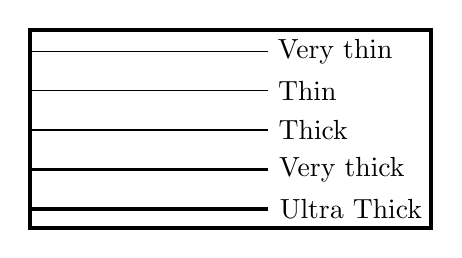
\begin{tikzpicture}[yscale=0.5]
\draw[very thin] (0,0) -- (3,0) node[right] {Very thin};
\draw[thin] (0,-1) -- (3,-1) node[right]{Thin};
\draw[thick] (0,-2) -- (3,-2) node[right]{Thick};
\draw[very thick] (0,-3) -- (3,-3) node[right]{Very thick};
\draw[ultra thick] (0,-4) -- (3,-4) node[right]{Ultra Thick};

\draw[ultra thick] (current bounding box.north east) rectangle (current bounding box.south west);

\end{tikzpicture}
\caption{Line Widths}
\end{figure}

%------------------

\begin{figure}[H]
\centering
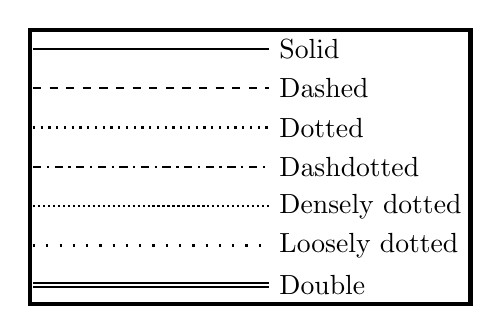
\begin{tikzpicture}[yscale=0.5]

\draw[thick,solid] (0,0) -- (3,0) node[right]{Solid};

\draw[thick,dashed] (0,-1) -- (3,-1) node[right]{Dashed};

\draw[thick,dotted] (0,-2) -- (3,-2) node[right]{Dotted};

\draw[thick,dashdotted] (0,-3) -- (3,-3) node[right] {Dashdotted};

\draw[thick,densely dotted] (0,-4) -- (3,-4) node[right] {Densely dotted};

\draw[thick,loosely dotted] (0,-5) -- (3,-5) node[right] {Loosely dotted};

\draw[thick,double] (0,-6) -- (3,-6) node[right] {Double};

\draw[ultra thick] (current bounding box.north east) rectangle (current bounding box.south west);
\end{tikzpicture}
\caption{Line Styles}
\end{figure}

%------------------
\begin{figure}[H]
\centering
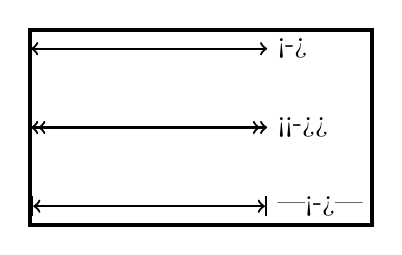
\begin{tikzpicture}[thick]
\draw[<->] (0,0) -- (3,0) node[right]{\lstinline{<->}};

\draw[<<->>] (0,-1) -- (3,-1) node[right]{\lstinline{<<->>}};

\draw[|<->|] (0,-2) -- (3,-2) node[right]{\lstinline{|<->|}};

%\draw[-*] (0,-3) -- (3,-3) node[right]{\lstinline{-*}};

\draw[ultra thick] (current bounding box.north east) rectangle (current bounding box.south west);
\end{tikzpicture}
\caption{Arrow Head Types}
\end{figure}



%------------------
\begin{figure}[H]
\centering
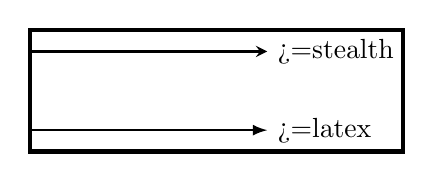
\begin{tikzpicture}[thick]

\draw[->,>=stealth] (0,0) -- (3,0) node[right]{\lstinline{>=stealth}};

\draw[->,>=latex] (0,-1) -- (3,-1) node[right]{\lstinline{>=latex}};


\draw[ultra thick] (current bounding box.north east) rectangle (current bounding box.south west);
\end{tikzpicture}
\caption{Arrow Header Styles}
\end{figure}


%% Rotational Circular Geometry

Figure \ref{Fig:rotationalcirculargeometry} shows rotational circular geometry typically seen in \textit{Dynamics}, drawn in TikZ.

\begin{figure}[H]
\centering
\begin{tikzpicture}[xscale=0.8,yscale=0.8]
% draw circle
\shadedraw[inner color=gray!10,outer color=gray!40, draw=black, very thick] (0,0) circle (3cm);

\tikzmath{
	\y = -45 + 90;
	\z = 90 - 45;
}

\draw[guide] (0,0) -- (\y:4cm);
\draw[guide] (0,0) -- (-45:5cm);
\draw[guide] (0,0) -- (5,0);

% phi-theta
\draw[->, very thick, blue] (5,0) arc (0:\z:5cm) node[label] {$\phi-\theta(t)$};

% phi
\draw [<-, very thick, space] (\y:4cm) arc (\y:-45:4cm) node[label] {$\phi$};

% theta
\draw[->, very thick] (5, 0) arc (0:-45:5cm) node[label] {$\theta(t)$};

% base vectors
%\draw[basevec] (\z:4cm) -- (\z:5cm);
%\draw[basevec] (\z:4cm) -- +(\z+90:1cm);
\nandm{45:4cm}{45}

% Points of interest
\poi{0,0}
\poi{-45:4cm}
\poi{5,0}

\end{tikzpicture}
\caption{Rotational Circular Geometry}
\label{Fig:rotationalcirculargeometry}
\end{figure}

% Rotate around
% Scope trick.
% https://tex.stackexchange.com/questions/19284/problem-when-drawing-an-axis-aligned-bounding-box-around-a-tilted-rectangle

Figure \ref{Fig:platonpin} shows how the idea of a \textit{scope} can be used to rotate objects in that scope about a point.

\begin{figure}[H]
\centering
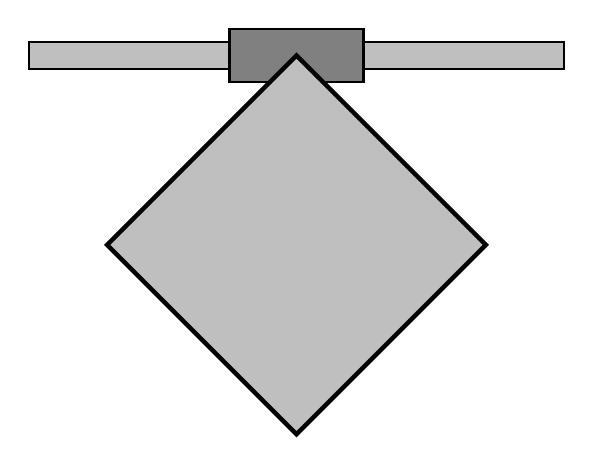
\begin{tikzpicture}[scale=1.7]
\centering

\shadedraw[top color=lightgray,middle color=gray,bottom color=lightgray,thick] (-2,-0.1) rectangle (2,0.1);
\draw[thick,fill=gray] (-0.5,-0.2) rectangle (0.5,0.2);

\begin{scope}[rotate around={-135:(0,0)}]
\draw[ultra thick,fill=lightgray] (0,0) rectangle (2,2);
\end{scope}
\poi{0,0}
%\poi{2,2}

\end{tikzpicture}
\caption{Rotating plate connected to pin}
\label{Fig:platonpin}
\end{figure}


Figure \ref{Fig:mulispringsys} is a multi-spring system drawn with TikZ. The springs are rendered using the \textit{stanli} package. The package offers a spring lifestyle.

% https://tex.stackexchange.com/questions/430943/latex-stanli-package-how-to-design-a-spring-element#430951
\begin{figure}[H]
\centering
\begin{tikzpicture}

\draw[thin,fill=lightgray] (0,-0.1) rectangle (9,0.1);

\begin{scope}
\draw[ultra thick,fill=gray] (2,-0.5) rectangle (3,0.5);
\draw[spring] (0,0) -- (2,0);
\end{scope}

\begin{scope}[xshift=3cm]
\draw[ultra thick,fill=gray] (2,-0.5) rectangle (3,0.5);
\draw[spring] (0,0) -- (2,0);
\end{scope}

\begin{scope}[xshift=6cm]
\draw[ultra thick,fill=gray] (2,-0.5) rectangle (3,0.5);
\draw[spring] (0,0) -- (2,0);
\end{scope}

%\filldraw[shading=axis,top color=gray, bottom color=white,line width=10pt, cap=round] (0,-1) --(2,-1);

\end{tikzpicture}
\caption{Drawing springs}
\label{Fig:mulispringsys}
\end{figure}


\begin{figure}
\centering
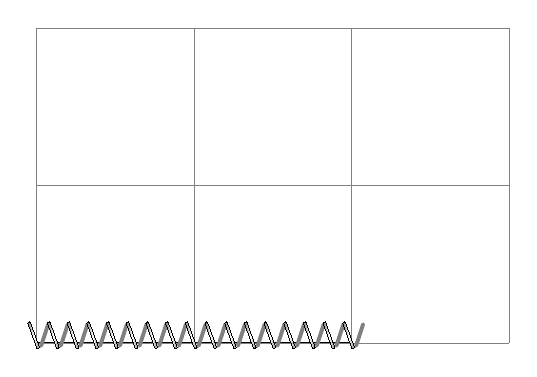
\begin{tikzpicture}[scale=2,decoration={
	markings,% switch on markings
	mark=% actually add a mark
	between positions 0 and 1 step 2.5mm with
{
	\begin{scope}[rotate around={110:(0,0)}]
		\shadedraw[rounded corners=0.2pt,
			right color=gray,
			left color= gray,
			middle color=white,
			line width=0
			]
		(-2pt,-0.5pt)
		rectangle
		(8pt,0.5pt);
	\end{scope}
	\begin{scope}[xshift=2pt,rotate around={72:(0,0)}]
		\filldraw[rounded corners=0.5pt, color=gray,fill=gray]
		(-1.5pt,-0.5pt)
		rectangle
		(7.5pt,0.5pt);
	\end{scope}
}
}
]
\draw [help lines] grid (3,2);
\draw [postaction={decorate}] (0,0) -- (2,0);
\end{tikzpicture}
\end{figure}



\begin{figure}
\centering
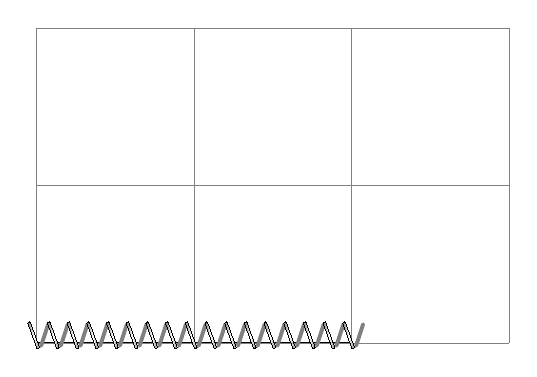
\begin{tikzpicture}[scale=2,decoration={
	markings,% switch on markings
	mark=% actually add a mark
	between positions 0 and 1 step 2.5mm with
{
	\begin{scope}[rotate around={110:(0,0)}]
		\shadedraw[rounded corners=0.2pt,
			right color=gray,
			left color= gray,
			middle color=white,
			line width=0
			]
		(-2pt,-0.5pt)
		rectangle
		(8pt,0.5pt);
	\end{scope}
	\begin{scope}[xshift=2pt,rotate around={72:(0,0)}]
		\filldraw[rounded corners=0.5pt, color=gray,fill=gray]
		(-1.5pt,-0.5pt)
		rectangle
		(7.5pt,0.5pt);
	\end{scope}
}
}
]
\draw [help lines] grid (3,2);
\draw [postaction={decorate}] (0,0) -- (2,0);
\end{tikzpicture}
\end{figure}











\end{appendices}

%---------------------------------------------

%% The following is for an optional glossary section

%\clearpage
%\glsaddall
%\printglossary[title={Variables Definitions}]

%% The following is for an optional references section

%\newpage
%\bibliography{References}
%\addcontentsline{toc}{section}{References}
%\bibliographystyle{apalike}
\end{document}
